% ------------------------------------------------------------------------------
% 6.2. ANÁLISIS DE CASOS DE USO
% ------------------------------------------------------------------------------
\subsection{6.2. Análisis de Casos de Uso}\label{sec:cap6_analisis_cu}

El análisis de cada caso de uso se realizó mediante diagramas de colaboración que representan las clases de análisis que intervienen y los mensajes que intercambian. Siguiendo el Proceso Unificado de Desarrollo de Software, el modelo de análisis distingue tres tipos de clases: las clases de interfaz (\textit{boundary}), que modelan la interacción del actor con el sistema; las clases de control (\textit{control}), que coordinan la lógica de cada caso de uso; y las clases de entidad (\textit{entity}), que representan la información persistente del dominio \parencite{jacobson1999unified}. Estos diagramas se expresan en el Lenguaje Unificado de Modelado \parencite{booch2005uml}.

En todos los diagramas, el actor se comunica con la interfaz (clase terminada en \textit{View}), esta con el controlador (clase terminada en \textit{Controller}) y el controlador con las entidades; no existe comunicación directa entre el actor y el controlador ni entre la interfaz y las entidades. Los mensajes se numeran jerárquicamente: el número entero corresponde a la operación que solicita el actor, y los subniveles (1.1, 1.2, etc.) a los mensajes que se derivan de ella hacia el controlador y las entidades. Las flechas se diferencian por color según el tipo de operación. Los nombres de las entidades se corresponden con las tablas del modelo de datos del sistema.

A continuación se presenta el análisis de los veintiséis casos de uso del sistema, en el orden de su numeración (CU-01 a CU-26).

\subsubsection{6.2.1. Analizar CU-01 Registrarse y autenticarse}\label{sec:cap6_analisis_cu01}

En el análisis del CU-01 participa el actor Usuario del Sistema, generalizado por los cuatro roles del sistema (Postulante, Administrador DUBSS, Directivo y Personal del Comedor Universitario), de modo que cualquiera de ellos puede registrarse o iniciar sesión. El actor interactúa con la interfaz \textit{AuthView}, que delega las solicitudes en el controlador \textit{AuthController}, y este accede a las entidades \textit{Usuario} y \textit{Postulante}. La Figura~\ref{fig:analisis_cu01} presenta el diagrama de análisis.

\begin{figure}[H]
\caption{Análisis del CU-01 Registrarse y autenticarse}
\label{fig:analisis_cu01}
\centering
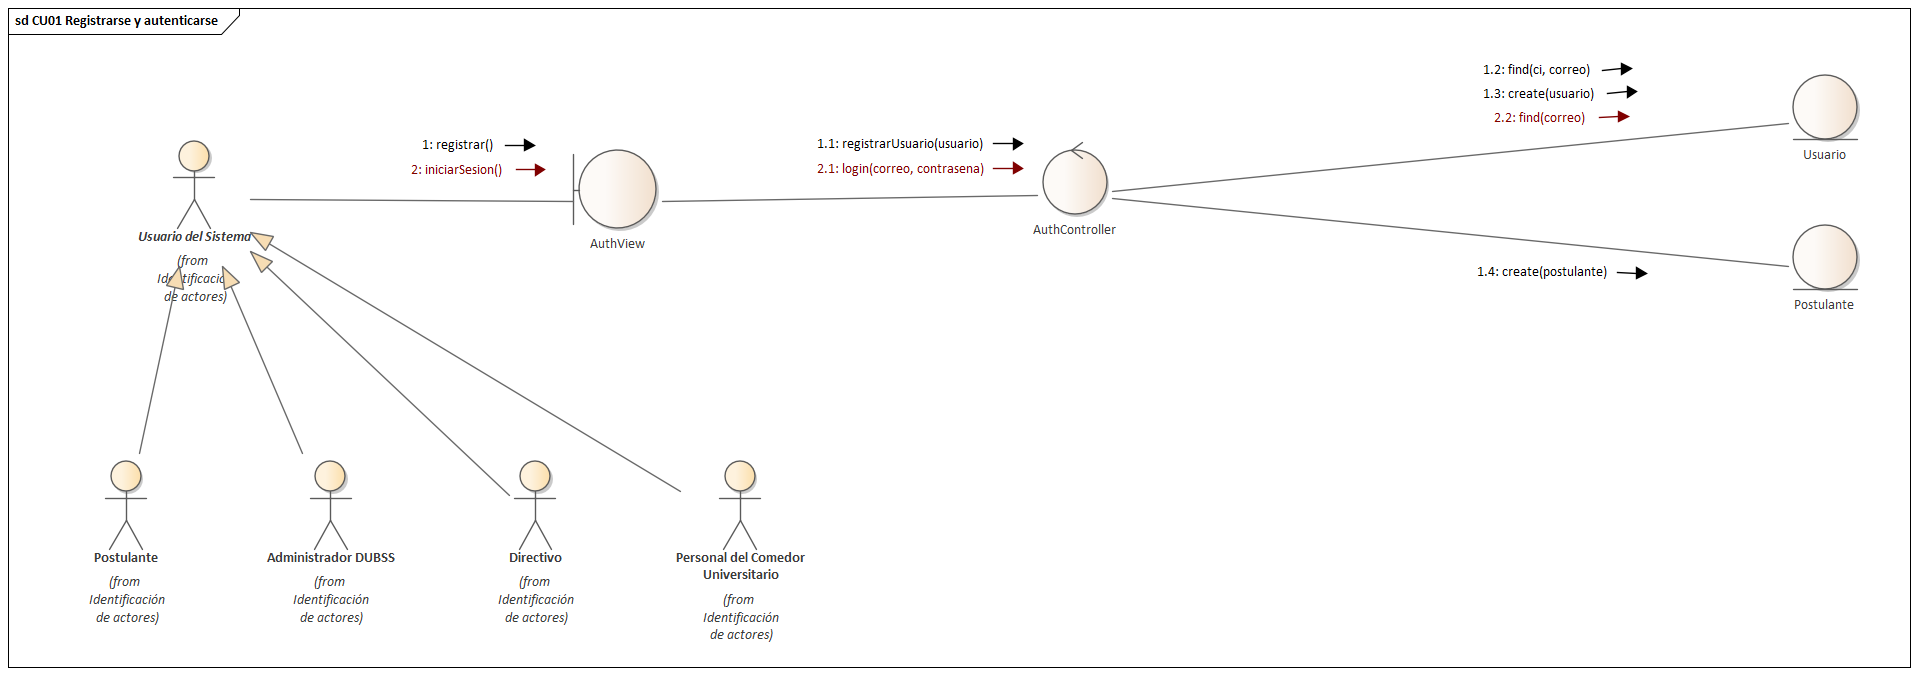
\includegraphics[width=\textwidth,height=0.5\textheight,keepaspectratio]{images/051_Analisis_CU01_Registrarse_Autenticarse.png}

\smallskip
\noindent\raggedright\textit{Nota.} Elaboración propia.
\end{figure}

El registro (mensaje 1) verifica que el CI y el correo electrónico no existan (1.2), crea el usuario (1.3) y, para el rol Postulante, crea su perfil (1.4). El inicio de sesión (mensaje 2) valida las credenciales consultando al usuario por su correo electrónico (2.2); si son válidas, el controlador emite el token JWT con el que se autentican las siguientes peticiones \parencite{rouse2018jwt}.


\subsubsection{6.2.2. Analizar CU-02 Enviar postulación a Beca Comedor}\label{sec:cap6_analisis_cu02}

El CU-02 es iniciado por el Postulante a través de \textit{PostulacionView}, que se comunica con \textit{PostulacionController}. Este controlador utiliza las entidades \textit{Convocatoria}, \textit{Postulacion} y \textit{RespuestaSocioeconomica}. La digitalización de documentos, la validación de elegibilidad y la precalificación se resuelven en los casos de uso incluidos (CU-16, CU-18 y CU-03), por lo que no se repiten en este diagrama. La Figura~\ref{fig:analisis_cu02} presenta el diagrama de análisis.

\begin{figure}[H]
\caption{Análisis del CU-02 Enviar postulación a Beca Comedor}
\label{fig:analisis_cu02}
\centering
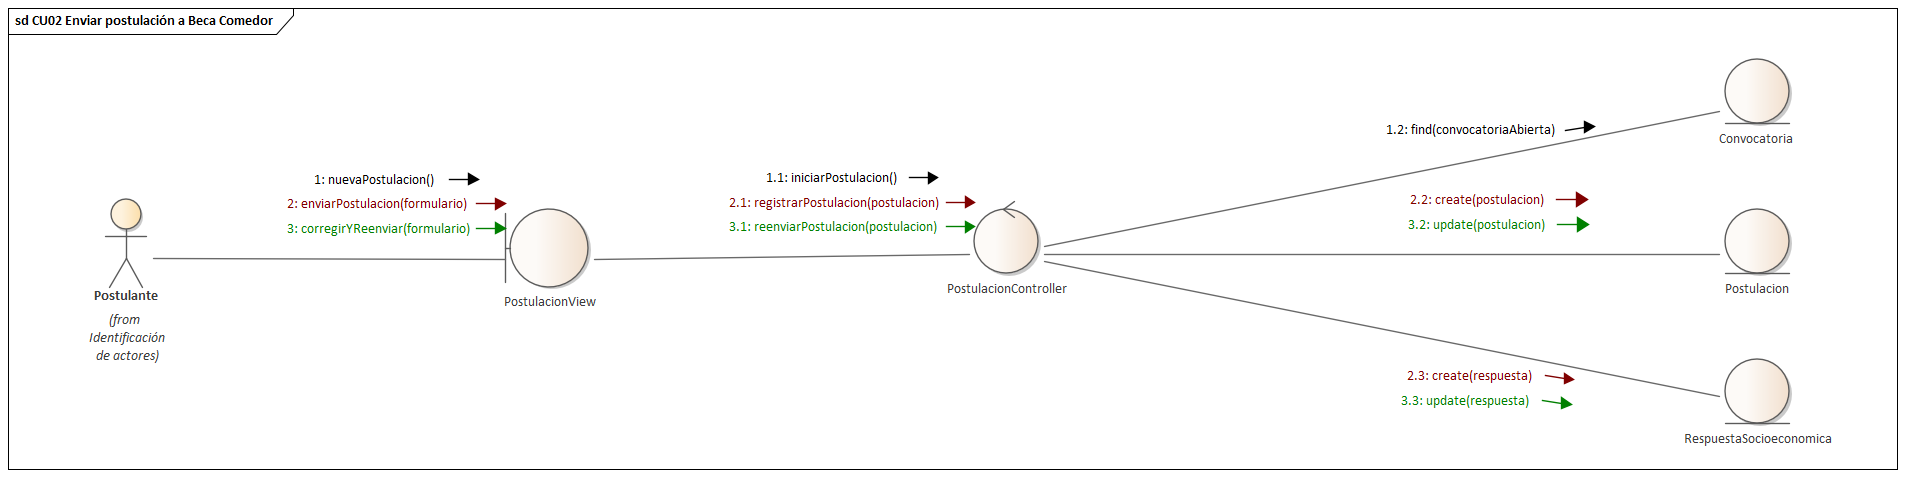
\includegraphics[width=\textwidth,height=0.5\textheight,keepaspectratio]{images/052_Analisis_CU02_Enviar_Postulacion_Beca_Comedor.png}

\smallskip
\noindent\raggedright\textit{Nota.} Elaboración propia.
\end{figure}

Al iniciar una nueva postulación (mensaje 1), el controlador consulta la convocatoria abierta (1.2). Al enviar el formulario (mensaje 2), crea la postulación (2.2) y su respuesta socioeconómica (2.3). Si la postulación fue devuelta para corrección, el Postulante la corrige y la reenvía (mensaje 3), con lo cual se actualizan la postulación (3.2) y la respuesta socioeconómica (3.3) sobre los mismos registros.


\subsubsection{6.2.3. Analizar CU-03 Precalificar postulación con Inteligencia Artificial}\label{sec:cap6_analisis_cu03}

El CU-03 se dispara cuando el Postulante envía su postulación desde \textit{PostulacionView}. El controlador \textit{PrecalificacionController} recibe la solicitud de precalificación y colabora con las entidades \textit{Postulacion}, \textit{ModeloPreseleccion}, \textit{ParametroModelo} y \textit{PuntajePostulacion}. El módulo de Inteligencia Artificial no se representa como objeto independiente: su ejecución se modela como el mensaje 1.5 del propio controlador. La Figura~\ref{fig:analisis_cu03} presenta el diagrama de análisis.

\begin{figure}[H]
\caption{Análisis del CU-03 Precalificar postulación con Inteligencia Artificial}
\label{fig:analisis_cu03}
\centering
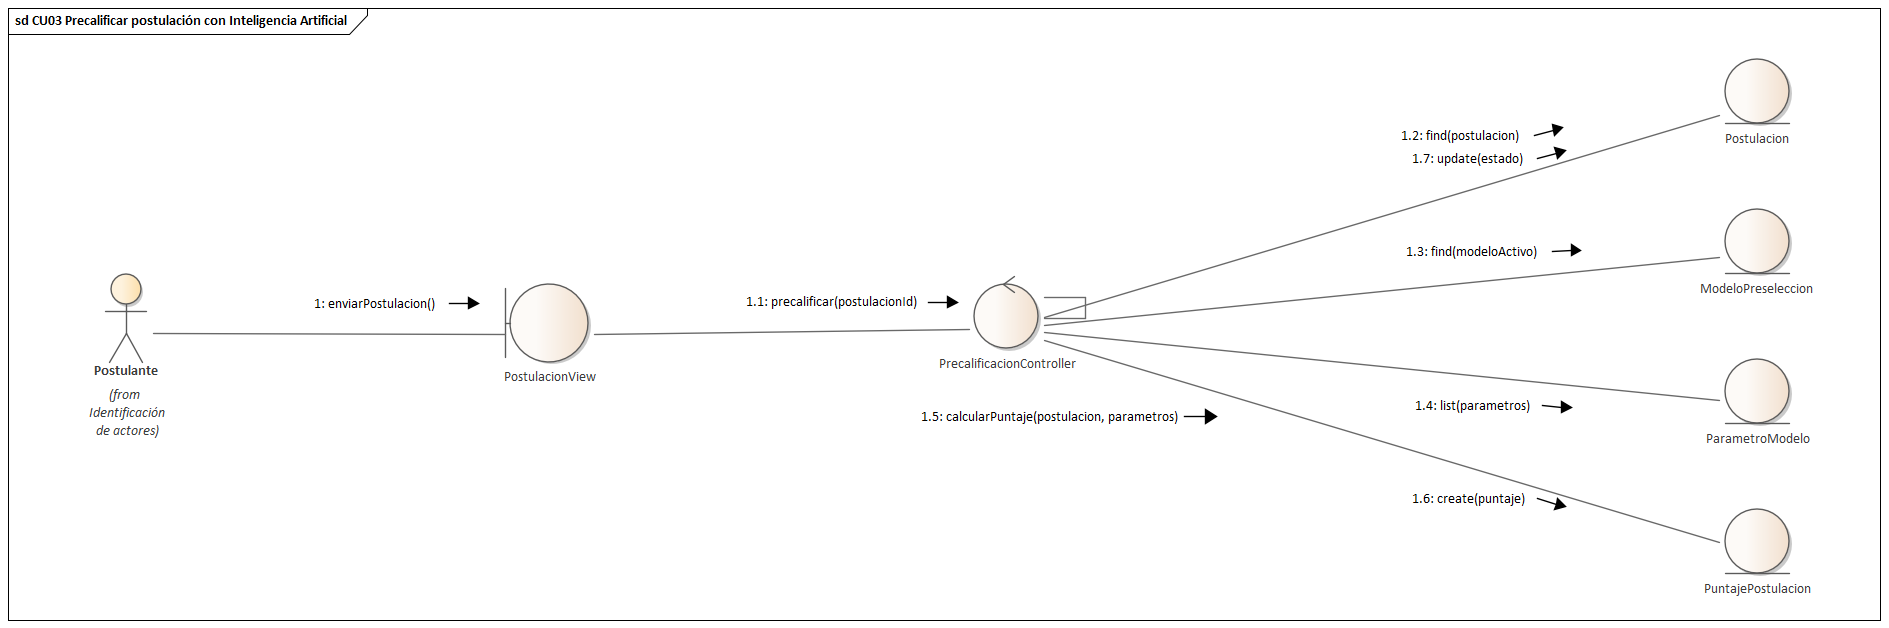
\includegraphics[width=\textwidth,height=0.5\textheight,keepaspectratio]{images/053_Analisis_CU03_Precalificar_Postulacion_IA.png}

\smallskip
\noindent\raggedright\textit{Nota.} Elaboración propia.
\end{figure}

El controlador obtiene la postulación (1.2), el modelo de preselección activo (1.3) y sus parámetros (1.4); calcula el puntaje de vulnerabilidad (1.5); registra el puntaje con su fecha de cálculo (1.6) y actualiza el estado de la postulación (1.7), lo que permite conservar la trazabilidad de cada cálculo.


\subsubsection{6.2.4. Analizar CU-04 Consultar estado de postulación}\label{sec:cap6_analisis_cu04}

En el CU-04, el Postulante consulta sus postulaciones mediante \textit{EstadoPostulacionView}, que se apoya en \textit{EstadoPostulacionController}. Las entidades involucradas son \textit{Postulacion} y \textit{PostulacionHistorial}. La Figura~\ref{fig:analisis_cu04} presenta el diagrama de análisis.

\begin{figure}[H]
\caption{Análisis del CU-04 Consultar estado de postulación}
\label{fig:analisis_cu04}
\centering
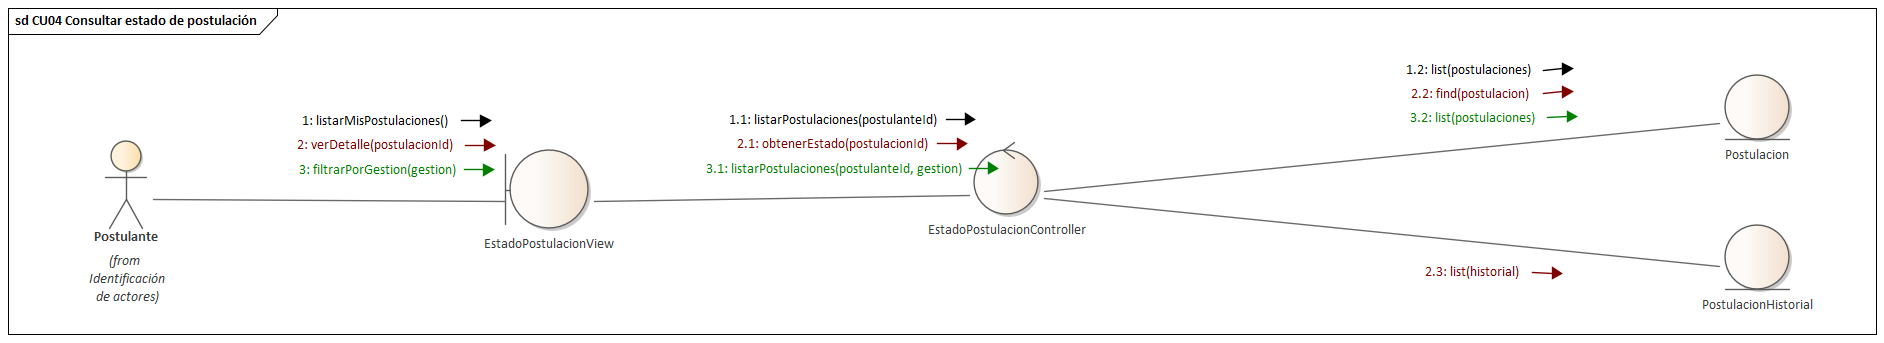
\includegraphics[width=\textwidth,height=0.5\textheight,keepaspectratio]{images/054_Analisis_CU04_Consultar_Estado_Postulacion.png}

\smallskip
\noindent\raggedright\textit{Nota.} Elaboración propia.
\end{figure}

El actor puede listar sus postulaciones (mensaje 1), ver el detalle de una de ellas (mensaje 2), lo que implica obtener la postulación (2.2) y su historial de cambios de estado (2.3), y filtrar las postulaciones por gestión académica (mensaje 3). Se trata de operaciones de solo lectura.


\subsubsection{6.2.5. Analizar CU-05 Auditar y adjudicar becas}\label{sec:cap6_analisis_cu05}

En el CU-05, el Administrador DUBSS conduce la adjudicación mediante \textit{AdjudicacionView}, que delega en \textit{AdjudicacionController}. Este controlador trabaja con las entidades \textit{Finalista}, \textit{Postulacion} y \textit{Adjudicacion}. La visualización de la lista priorizada y la auditoría de cada expediente se resuelven en los casos de uso incluidos (CU-06 y CU-07), por lo que no se repiten en este diagrama. La Figura~\ref{fig:analisis_cu05} presenta el diagrama de análisis.

\begin{figure}[H]
\caption{Análisis del CU-05 Auditar y adjudicar becas}
\label{fig:analisis_cu05}
\centering
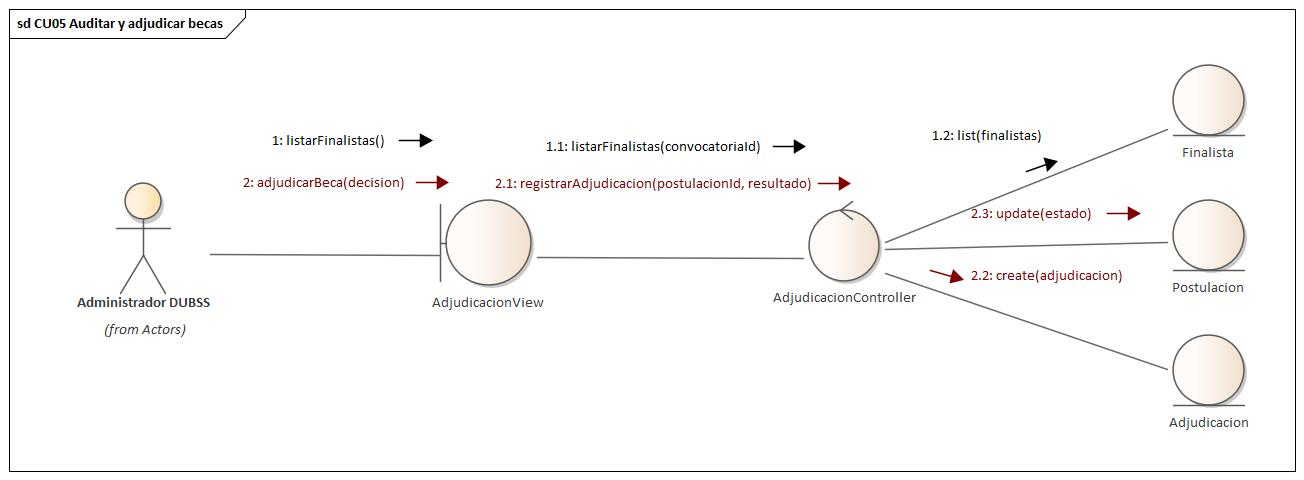
\includegraphics[width=\textwidth,height=0.5\textheight,keepaspectratio]{images/077_Analisis_CU05_Auditar_Adjudicar_Becas.jpg}

\smallskip
\noindent\raggedright\textit{Nota.} Elaboración propia.
\end{figure}

El Administrador puede listar los finalistas de la convocatoria (mensaje 1), con lo que el controlador obtiene los finalistas registrados (1.2). Al adjudicar una beca (mensaje 2), el controlador registra la decisión (2.1), crea la adjudicación con su resultado (2.2) y actualiza el estado de la postulación a «adjudicada» o «no adjudicada» (2.3).


\subsubsection{6.2.6. Analizar CU-06 Visualizar lista priorizada de postulantes}\label{sec:cap6_analisis_cu06}

En el CU-06, el Administrador DUBSS consulta la lista priorizada mediante \textit{ListaPriorizadaView}, que se comunica con \textit{PriorizacionController}. Las entidades involucradas son \textit{Postulacion} y \textit{PuntajePostulacion}; la lista no se almacena, sino que se obtiene a partir de ambas. La Figura~\ref{fig:analisis_cu06} presenta el diagrama de análisis.

\begin{figure}[H]
\caption{Análisis del CU-06 Visualizar lista priorizada de postulantes}
\label{fig:analisis_cu06}
\centering
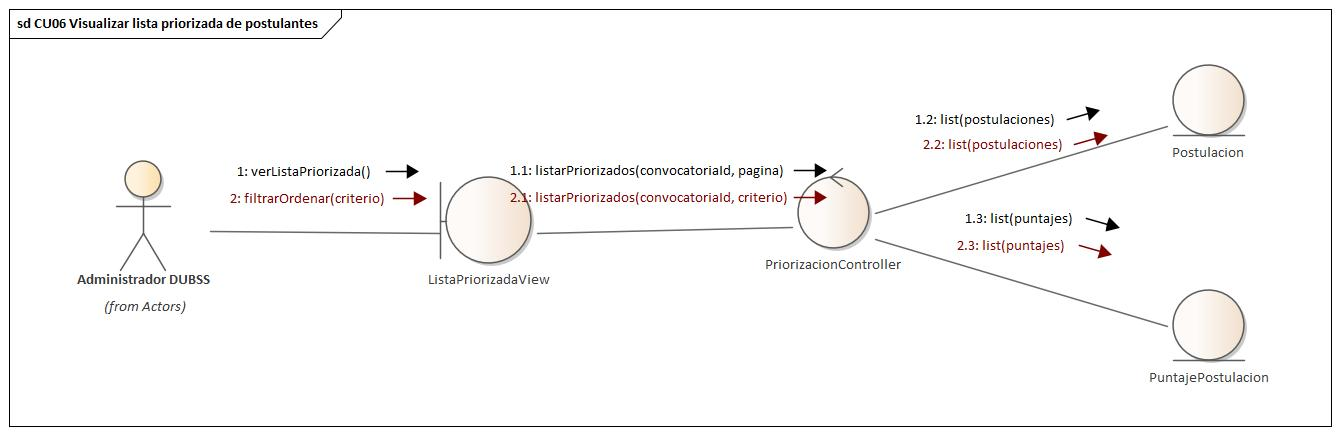
\includegraphics[width=\textwidth,height=0.5\textheight,keepaspectratio]{images/078_Analisis_CU06_Visualizar_Lista_Priorizada_Postulantes.jpg}

\smallskip
\noindent\raggedright\textit{Nota.} Elaboración propia.
\end{figure}

Al ver la lista priorizada (mensaje 1), el controlador solicita la página correspondiente de la convocatoria (1.1), obtiene las postulaciones calificadas (1.2) y sus puntajes vigentes (1.3), y las ordena de mayor a menor puntaje. Al filtrar u ordenar la lista (mensaje 2), se repite la consulta con el criterio indicado (2.1 a 2.3). Ambas operaciones son de solo lectura.


\subsubsection{6.2.7. Analizar CU-07 Auditar expediente finalista}\label{sec:cap6_analisis_cu07}

En el CU-07, el Administrador DUBSS revisa el expediente de un finalista mediante \textit{ExpedienteView} y \textit{ExpedienteController}, que colaboran con las entidades \textit{Finalista}, \textit{DocumentoAdjunto} y \textit{AuditoriaExpediente}. La notificación al finalista y el registro de la entrega física se resuelven en el CU-21, incluido por este caso de uso. La Figura~\ref{fig:analisis_cu07} presenta el diagrama de análisis.

\begin{figure}[H]
\caption{Análisis del CU-07 Auditar expediente finalista}
\label{fig:analisis_cu07}
\centering
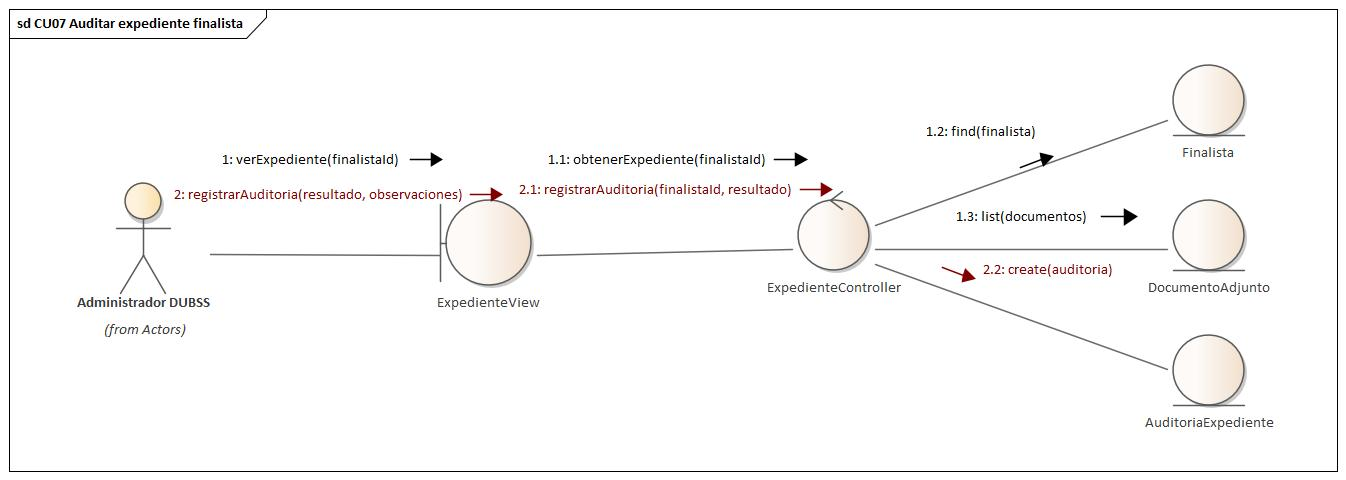
\includegraphics[width=\textwidth,height=0.5\textheight,keepaspectratio]{images/079_Analisis_CU07_Auditar_Expediente_Finalista.jpg}

\smallskip
\noindent\raggedright\textit{Nota.} Elaboración propia.
\end{figure}

Al ver el expediente (mensaje 1), el controlador obtiene el finalista (1.2) y la lista de sus documentos adjuntos (1.3). Al registrar la auditoría (mensaje 2), el controlador recibe el resultado (2.1) y crea el registro de auditoría con su resultado y observaciones (2.2), conservando las auditorías anteriores del expediente.


\subsubsection{6.2.8. Analizar CU-08 Generar acta de adjudicación}\label{sec:cap6_analisis_cu08}

En el CU-08, el Administrador DUBSS genera el acta mediante \textit{ActaView} y \textit{ActaController}, que utiliza las entidades \textit{Adjudicacion} y \textit{ActaAdjudicacion}. La generación del documento PDF se modela como un mensaje del propio controlador (1.3). La Figura~\ref{fig:analisis_cu08} presenta el diagrama de análisis.

\begin{figure}[H]
\caption{Análisis del CU-08 Generar acta de adjudicación}
\label{fig:analisis_cu08}
\centering
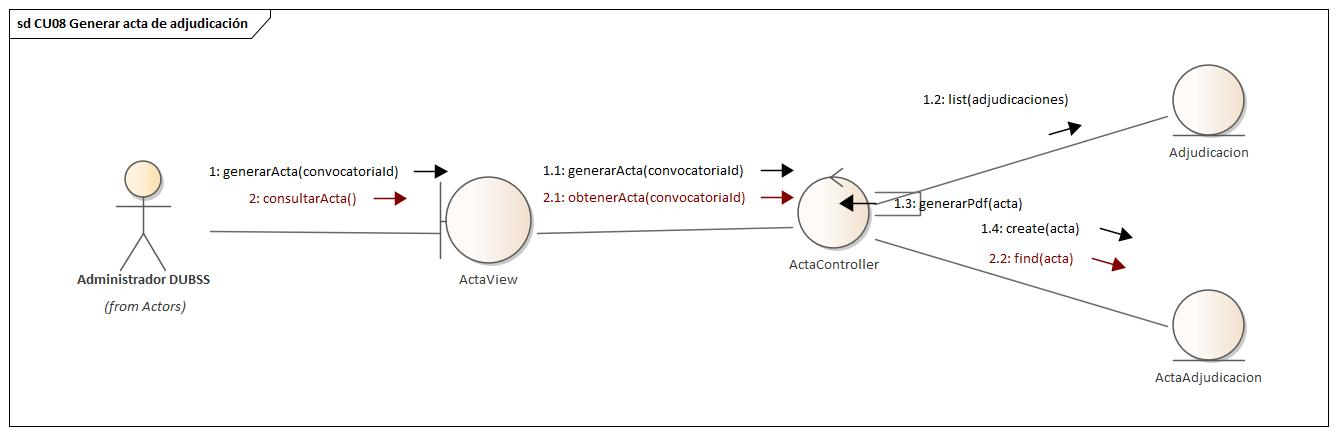
\includegraphics[width=\textwidth,height=0.5\textheight,keepaspectratio]{images/080_Analisis_CU08_Generar_Acta_Adjudicacion.jpg}

\smallskip
\noindent\raggedright\textit{Nota.} Elaboración propia.
\end{figure}

Al generar el acta (mensaje 1), el controlador obtiene las adjudicaciones de la convocatoria (1.2), genera el documento PDF (1.3) y crea el registro del acta (1.4). Al consultar el acta (mensaje 2), el controlador obtiene el acta registrada de la convocatoria (2.2).


\subsubsection{6.2.9. Analizar CU-09 Generar planilla de asistencia}\label{sec:cap6_analisis_cu09}

En el CU-09, el Administrador DUBSS genera las planillas mediante \textit{PlanillaView} y \textit{PlanillaController}, que trabajan con las entidades \textit{Beca} y \textit{PlanillaAsistencia}. La generación del documento PDF imprimible se modela como un mensaje del propio controlador (1.3). La Figura~\ref{fig:analisis_cu09} presenta el diagrama de análisis.

\begin{figure}[H]
\caption{Análisis del CU-09 Generar planilla de asistencia}
\label{fig:analisis_cu09}
\centering
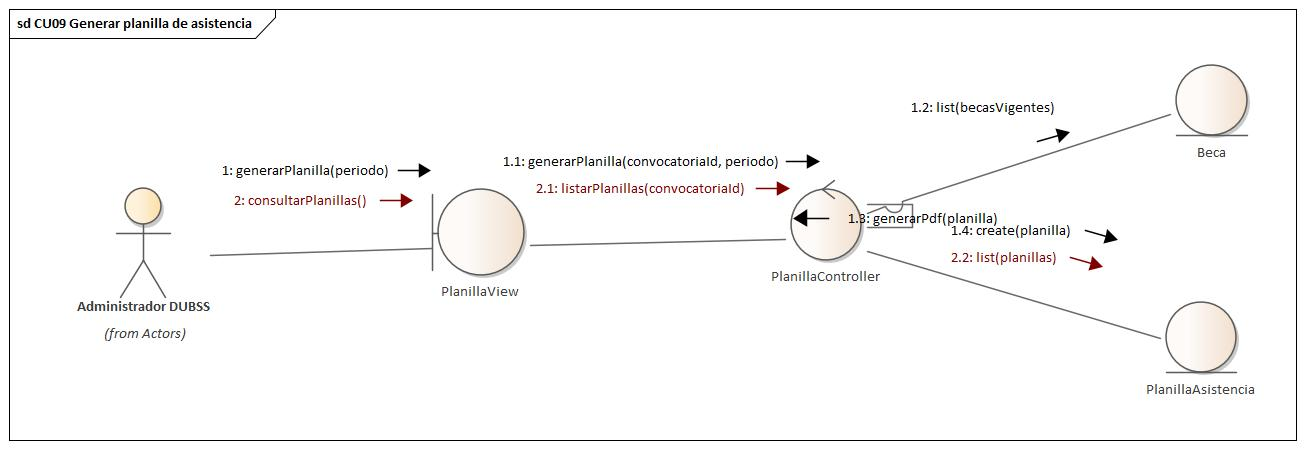
\includegraphics[width=\textwidth,height=0.5\textheight,keepaspectratio]{images/081_Analisis_CU09_Generar_Planilla_Asistencia.jpg}

\smallskip
\noindent\raggedright\textit{Nota.} Elaboración propia.
\end{figure}

Al generar una planilla para un periodo (mensaje 1), el controlador obtiene las becas vigentes de la convocatoria (1.2), genera el PDF con los espacios de firma y fotocopia de carnet (1.3) y crea el registro de la planilla (1.4). Al consultar las planillas (mensaje 2), el controlador lista las planillas generadas para la convocatoria (2.2).


\subsubsection{6.2.10. Analizar CU-10 Registrar asistencia digital}\label{sec:cap6_analisis_cu10}

En el CU-10, el Personal del Comedor Universitario registra la asistencia desde la aplicación móvil mediante \textit{RegistrarAsistenciaView}, que delega en \textit{AsistenciaControllerMobile}. Las entidades involucradas son \textit{Beca} y \textit{Asistencia}. La Figura~\ref{fig:analisis_cu10} presenta el diagrama de análisis.

\begin{figure}[H]
\caption{Análisis del CU-10 Registrar asistencia digital}
\label{fig:analisis_cu10}
\centering
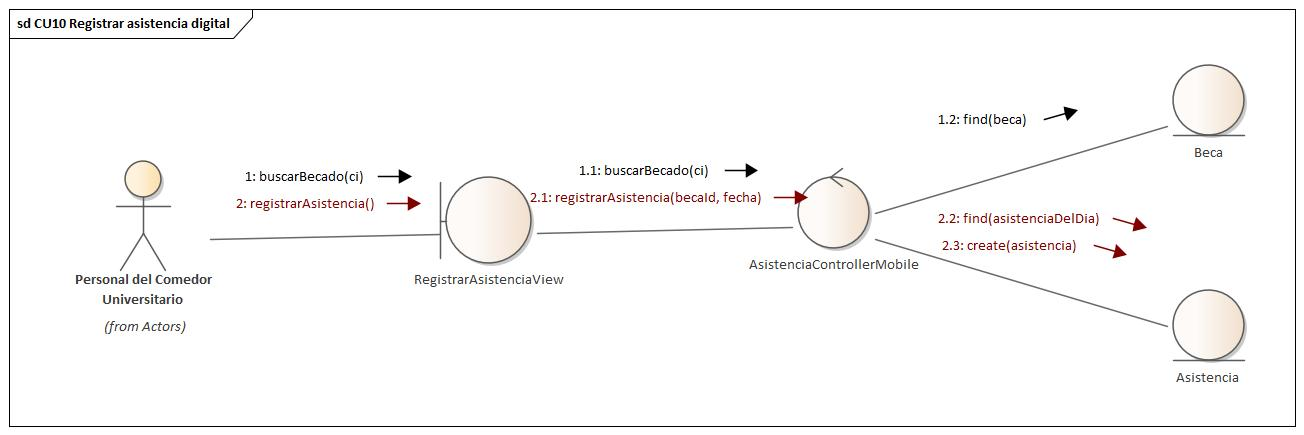
\includegraphics[width=\textwidth,height=0.5\textheight,keepaspectratio]{images/082_Analisis_CU10_Registrar_Asistencia_Digital.jpg}

\smallskip
\noindent\raggedright\textit{Nota.} Elaboración propia.
\end{figure}

Al buscar al becado por su CI (mensaje 1), el controlador obtiene su beca (1.2) para verificar que esté vigente. Al registrar la asistencia (mensaje 2), el controlador verifica si ya existe una asistencia de esa beca en el día (2.2) y, si no existe, crea el registro de asistencia (2.3); de este modo, una petición duplicada no genera un segundo registro.


\subsubsection{6.2.11. Analizar CU-11 Cotejar registro contra respaldo físico}\label{sec:cap6_analisis_cu11}

En el CU-11, el Administrador DUBSS realiza el cotejo mediante \textit{CotejoView} y \textit{CotejoController}, que colaboran con las entidades \textit{PlanillaAsistencia}, \textit{Asistencia} y \textit{CotejoAsistencia}. La Figura~\ref{fig:analisis_cu11} presenta el diagrama de análisis.

\begin{figure}[H]
\caption{Análisis del CU-11 Cotejar registro contra respaldo físico}
\label{fig:analisis_cu11}
\centering
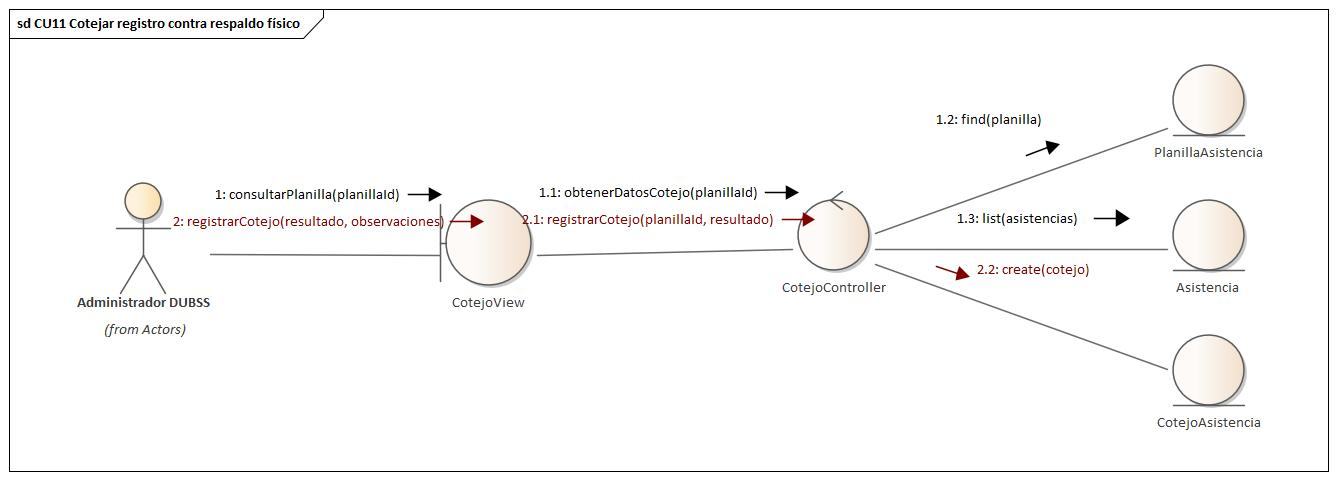
\includegraphics[width=\textwidth,height=0.5\textheight,keepaspectratio]{images/083_Analisis_CU11_Cotejar_Registro_Respaldo_Fisico.jpg}

\smallskip
\noindent\raggedright\textit{Nota.} Elaboración propia.
\end{figure}

Al consultar una planilla (mensaje 1), el controlador obtiene la planilla (1.2) y la lista de asistencias registradas en su periodo (1.3). Al registrar el cotejo (mensaje 2), el controlador recibe el resultado (2.1) y crea el registro del cotejo (2.2), sin modificar los registros de asistencia.


\subsubsection{6.2.12. Analizar CU-12 Visualizar dashboard de indicadores BI}\label{sec:cap6_analisis_cu12}

En el CU-12, el Directivo consulta el dashboard mediante \textit{DashboardView} y \textit{DashboardController}. La única entidad involucrada es \textit{IndicadoresConvocatoria}, que representa los indicadores precalculados por lotes a partir de las postulaciones, adjudicaciones, becas y asistencias. La Figura~\ref{fig:analisis_cu12} presenta el diagrama de análisis.

\begin{figure}[H]
\caption{Análisis del CU-12 Visualizar dashboard de indicadores BI}
\label{fig:analisis_cu12}
\centering
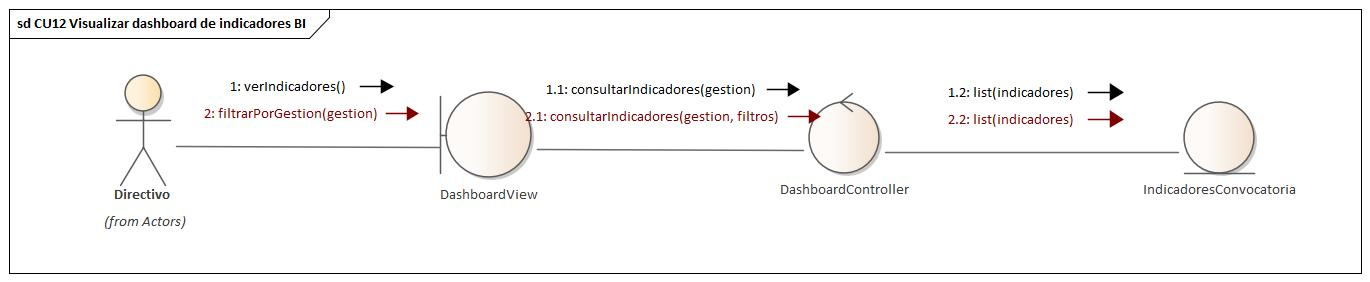
\includegraphics[width=\textwidth,height=0.5\textheight,keepaspectratio]{images/084_Analisis_CU12_Visualizar_Dashboard_Indicadores_BI.jpg}

\smallskip
\noindent\raggedright\textit{Nota.} Elaboración propia.
\end{figure}

Al ver los indicadores (mensaje 1), el controlador los consulta para la gestión académica vigente (1.1) y obtiene la lista de indicadores (1.2). Al filtrar por gestión (mensaje 2), se repite la consulta con la gestión y los filtros seleccionados (2.1 y 2.2). Ambas operaciones son de solo lectura.


\subsubsection{6.2.13. Analizar CU-13 Gestionar convocatoria y gestión académica}\label{sec:cap6_analisis_cu13}

En el CU-13, el Administrador DUBSS gestiona las convocatorias mediante \textit{ConvocatoriaView} y \textit{ConvocatoriaController}, que trabajan con las entidades \textit{Convocatoria}, \textit{GestionAcademica} y \textit{ConvocatoriaDocumento}. La Figura~\ref{fig:analisis_cu13} presenta el diagrama de análisis.

\begin{figure}[H]
\caption{Análisis del CU-13 Gestionar convocatoria y gestión académica}
\label{fig:analisis_cu13}
\centering
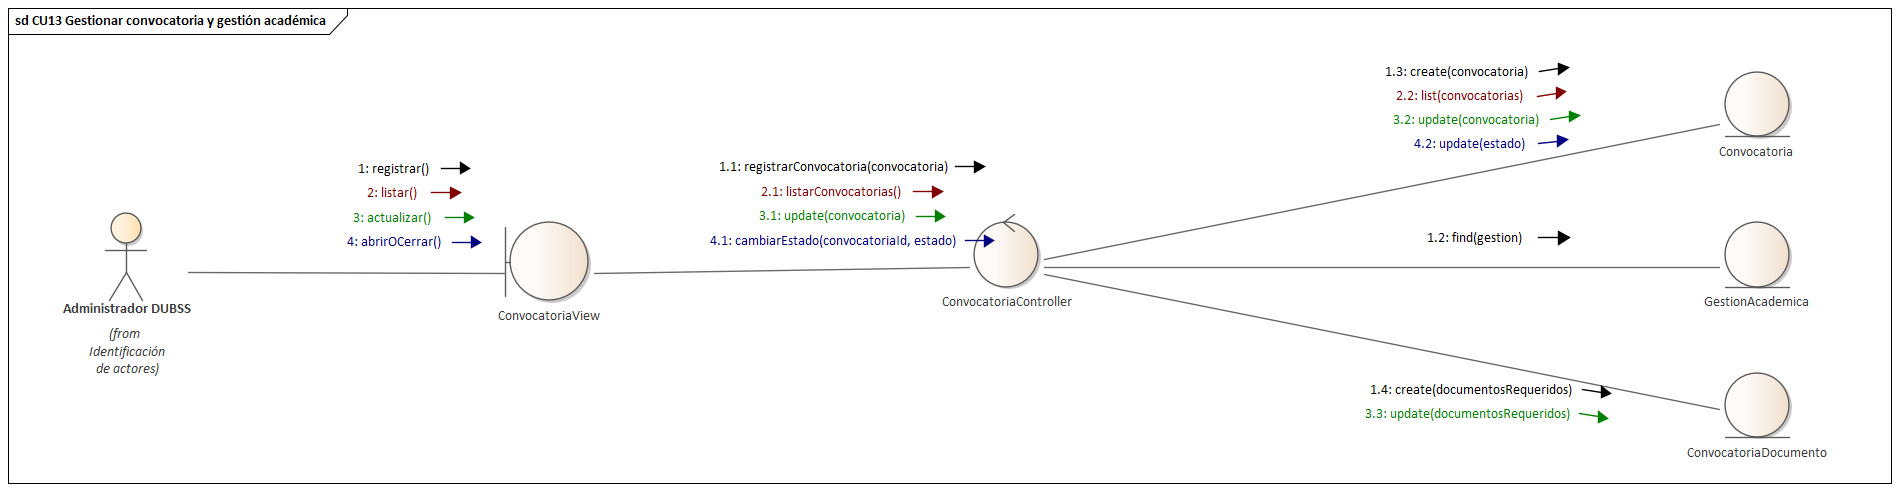
\includegraphics[width=\textwidth,height=0.5\textheight,keepaspectratio]{images/055_Analisis_CU13_Gestionar_Convocatoria_Gestion_Academica.png}

\smallskip
\noindent\raggedright\textit{Nota.} Elaboración propia.
\end{figure}

El registro de una convocatoria (mensaje 1) consulta la gestión académica (1.2), crea la convocatoria (1.3) y crea la lista de documentos requeridos (1.4). El listado (mensaje 2) recupera las convocatorias (2.2). La actualización (mensaje 3) modifica la convocatoria (3.2) y sus documentos requeridos (3.3). Finalmente, abrir o cerrar una convocatoria (mensaje 4) actualiza su estado (4.2). No se incluye una operación de eliminación, pues una convocatoria con postulaciones asociadas solo puede cerrarse.


\subsubsection{6.2.14. Analizar CU-14 Gestionar usuarios y roles}\label{sec:cap6_analisis_cu14}

En el CU-14, el Administrador DUBSS administra las cuentas del personal mediante \textit{UsuarioView} y \textit{UsuarioController}, que utilizan las entidades \textit{Usuario} y \textit{Rol}. La Figura~\ref{fig:analisis_cu14} presenta el diagrama de análisis.

\begin{figure}[H]
\caption{Análisis del CU-14 Gestionar usuarios y roles}
\label{fig:analisis_cu14}
\centering
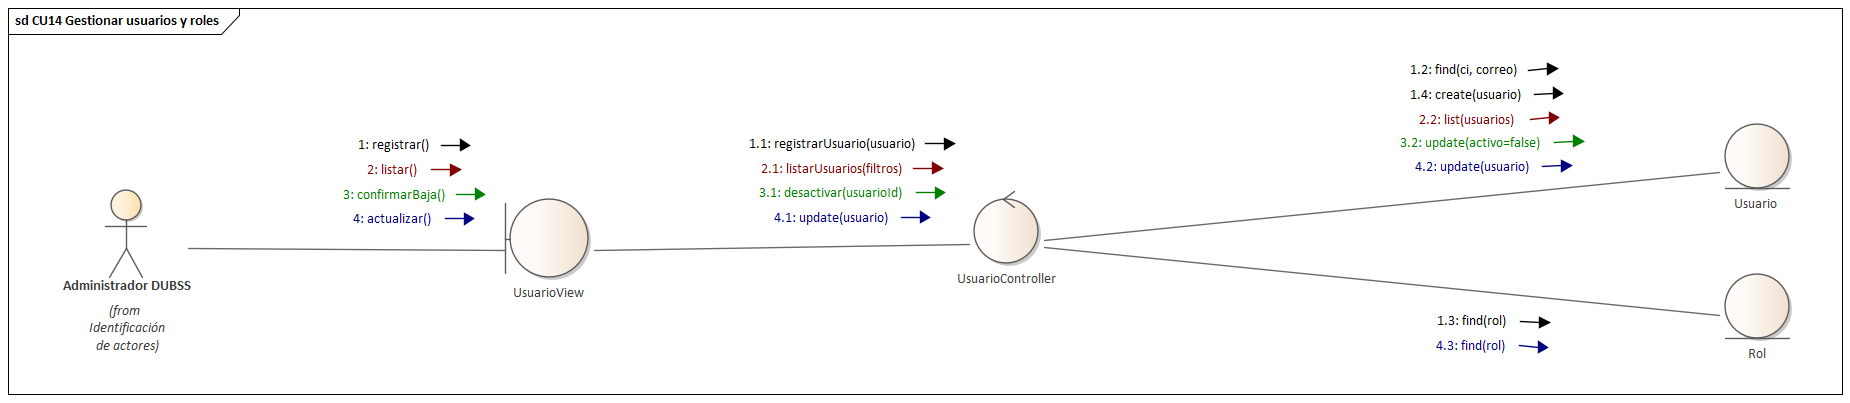
\includegraphics[width=\textwidth,height=0.5\textheight,keepaspectratio]{images/056_Analisis_CU14_Gestionar_Usuarios_Roles.png}

\smallskip
\noindent\raggedright\textit{Nota.} Elaboración propia.
\end{figure}

Para registrar una cuenta (mensaje 1), el controlador verifica que el CI y el correo no existan (1.2), consulta el rol asignado (1.3) y crea el usuario (1.4). El listado (mensaje 2) recupera los usuarios según los filtros indicados (2.2). La baja (mensaje 3) desactiva la cuenta mediante la actualización del campo de actividad (3.2), sin eliminar el registro, de modo que se preserve la trazabilidad. La actualización (mensaje 4) modifica los datos del usuario (4.2) y su rol (4.3).


\subsubsection{6.2.15. Analizar CU-15 Recuperar contraseña / gestionar perfil}\label{sec:cap6_analisis_cu15}

En el CU-15 participa el actor Usuario del Sistema, generalizado por los cuatro roles, quien interactúa con \textit{PerfilView}. El controlador \textit{PerfilController} colabora con las entidades \textit{Usuario}, \textit{Postulante} y \textit{TokenRestablecimiento}. La Figura~\ref{fig:analisis_cu15} presenta el diagrama de análisis.

\begin{figure}[H]
\caption{Análisis del CU-15 Recuperar contraseña / gestionar perfil}
\label{fig:analisis_cu15}
\centering
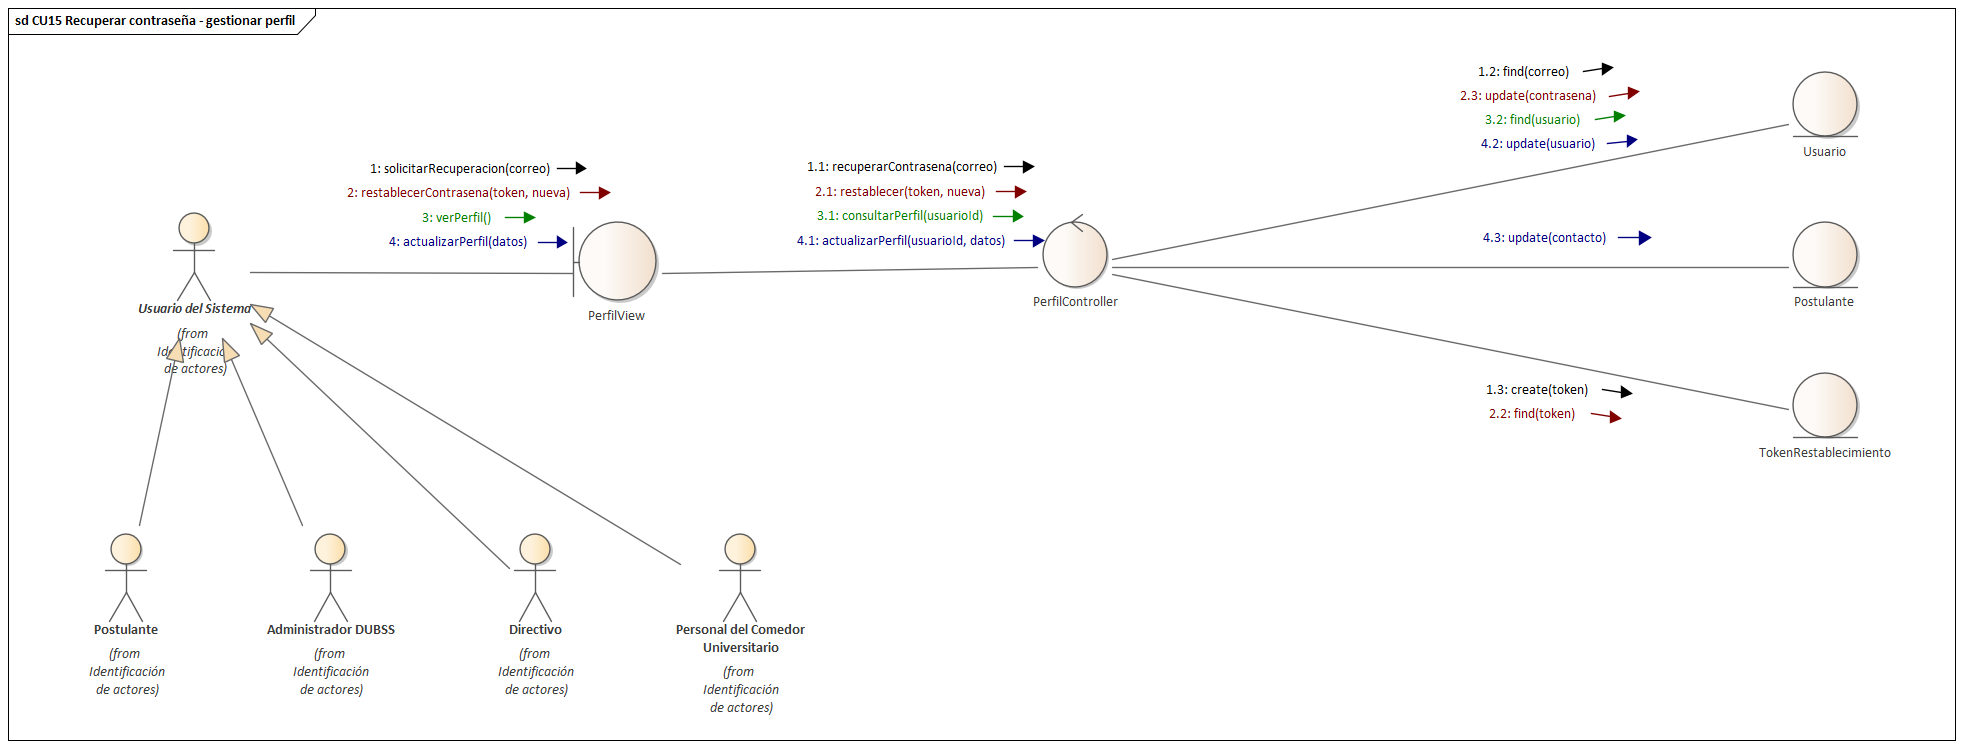
\includegraphics[width=\textwidth,height=0.5\textheight,keepaspectratio]{images/057_Analisis_CU15_Recuperar_Contrasena_Gestionar_Perfil.png}

\smallskip
\noindent\raggedright\textit{Nota.} Elaboración propia.
\end{figure}

La solicitud de recuperación (mensaje 1) consulta al usuario por su correo (1.2) y genera un token de restablecimiento de un solo uso (1.3). El restablecimiento (mensaje 2) verifica el token (2.2) y actualiza la contraseña del usuario (2.3). La consulta del perfil (mensaje 3) obtiene los datos del usuario (3.2) y su actualización (mensaje 4) modifica los datos del usuario (4.2) y los datos de contacto del postulante (4.3).


\subsubsection{6.2.16. Analizar CU-16 Digitalizar y adjuntar documentos}\label{sec:cap6_analisis_cu16}

En el CU-16, el Postulante adjunta los documentos de respaldo mediante \textit{DocumentoView} y \textit{DocumentoController}, que utilizan las entidades \textit{ConvocatoriaDocumento} y \textit{DocumentoAdjunto}. La Figura~\ref{fig:analisis_cu16} presenta el diagrama de análisis.

\begin{figure}[H]
\caption{Análisis del CU-16 Digitalizar y adjuntar documentos}
\label{fig:analisis_cu16}
\centering
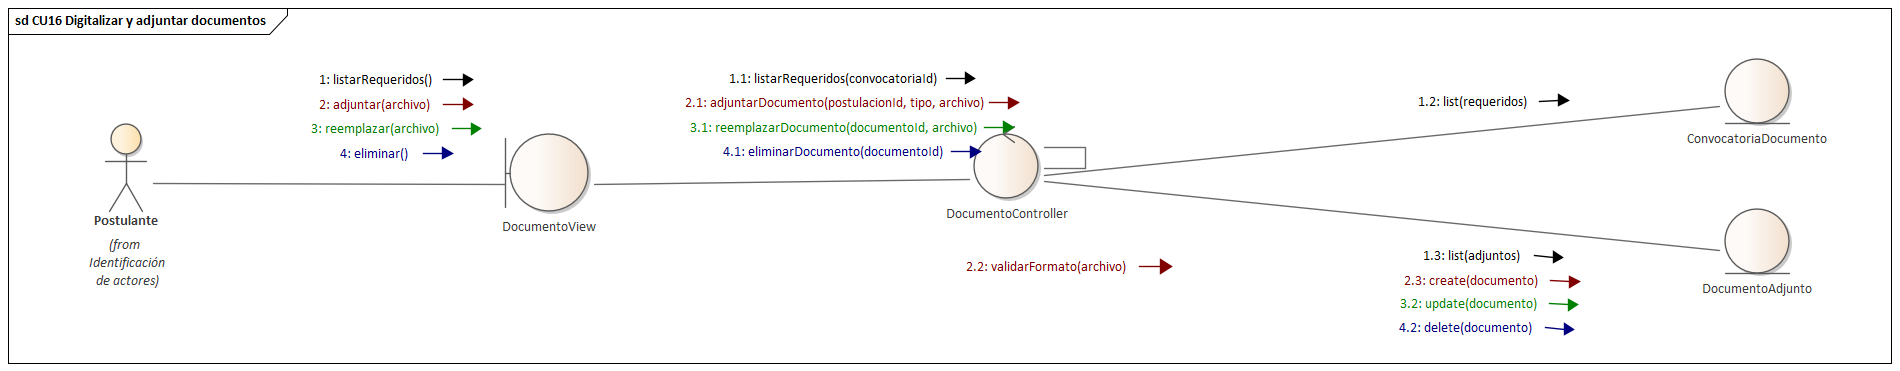
\includegraphics[width=\textwidth,height=0.5\textheight,keepaspectratio]{images/058_Analisis_CU16_Digitalizar_Adjuntar_Documentos.png}

\smallskip
\noindent\raggedright\textit{Nota.} Elaboración propia.
\end{figure}

Primero se listan los documentos requeridos por la convocatoria y los ya adjuntados (mensaje 1, con los pasos 1.2 y 1.3). Al adjuntar un archivo (mensaje 2), el controlador valida su formato (2.2) y crea el documento adjunto (2.3). El reemplazo (mensaje 3) actualiza el documento (3.2) y la eliminación (mensaje 4) lo elimina (4.2), operaciones permitidas antes del envío de la postulación o cuando esta fue devuelta.


\subsubsection{6.2.17. Analizar CU-17 Guardar borrador de postulación}\label{sec:cap6_analisis_cu17}

En el CU-17, el Postulante guarda y retoma su postulación incompleta mediante \textit{BorradorView} y \textit{BorradorController}, que trabajan con las entidades \textit{Convocatoria}, \textit{Postulacion} y \textit{RespuestaSocioeconomica}. La Figura~\ref{fig:analisis_cu17} presenta el diagrama de análisis.

\begin{figure}[H]
\caption{Análisis del CU-17 Guardar borrador de postulación}
\label{fig:analisis_cu17}
\centering
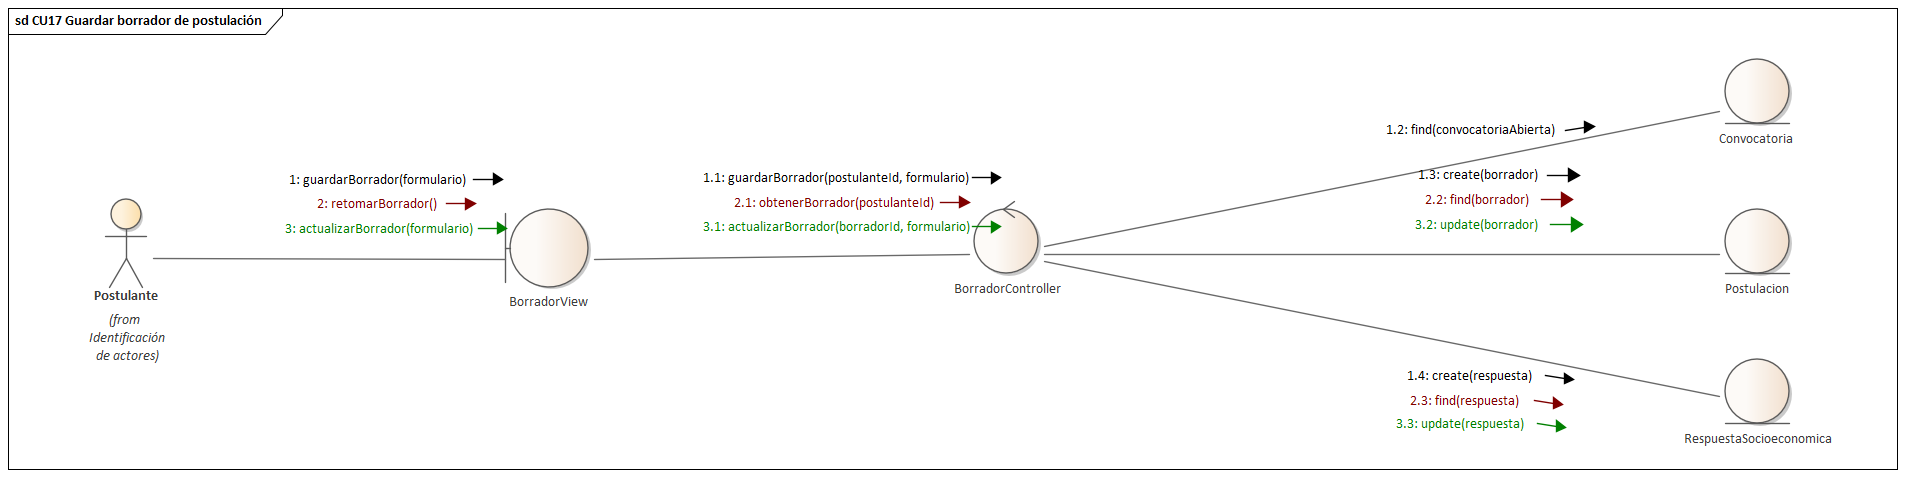
\includegraphics[width=\textwidth,height=0.5\textheight,keepaspectratio]{images/059_Analisis_CU17_Guardar_Borrador_Postulacion.png}

\smallskip
\noindent\raggedright\textit{Nota.} Elaboración propia.
\end{figure}

Al guardar el borrador (mensaje 1), el controlador verifica que la convocatoria esté abierta (1.2) y crea la postulación en estado de borrador (1.3) con las respuestas ingresadas (1.4), sin exigir los campos obligatorios. Al retomarlo (mensaje 2) se recuperan el borrador (2.2) y sus respuestas (2.3), y al continuar editándolo (mensaje 3) se actualizan ambos (3.2 y 3.3). El borrador no se envía al módulo de precalificación.


\subsubsection{6.2.18. Analizar CU-18 Validar elegibilidad y duplicados}\label{sec:cap6_analisis_cu18}

El CU-18 es incluido por el CU-02: se ejecuta cuando el Postulante envía su postulación a través de \textit{PostulacionView}. El controlador \textit{ValidacionController} colabora con las entidades \textit{Postulante}, \textit{Convocatoria} y \textit{Postulacion}. La Figura~\ref{fig:analisis_cu18} presenta el diagrama de análisis.

\begin{figure}[H]
\caption{Análisis del CU-18 Validar elegibilidad y duplicados}
\label{fig:analisis_cu18}
\centering
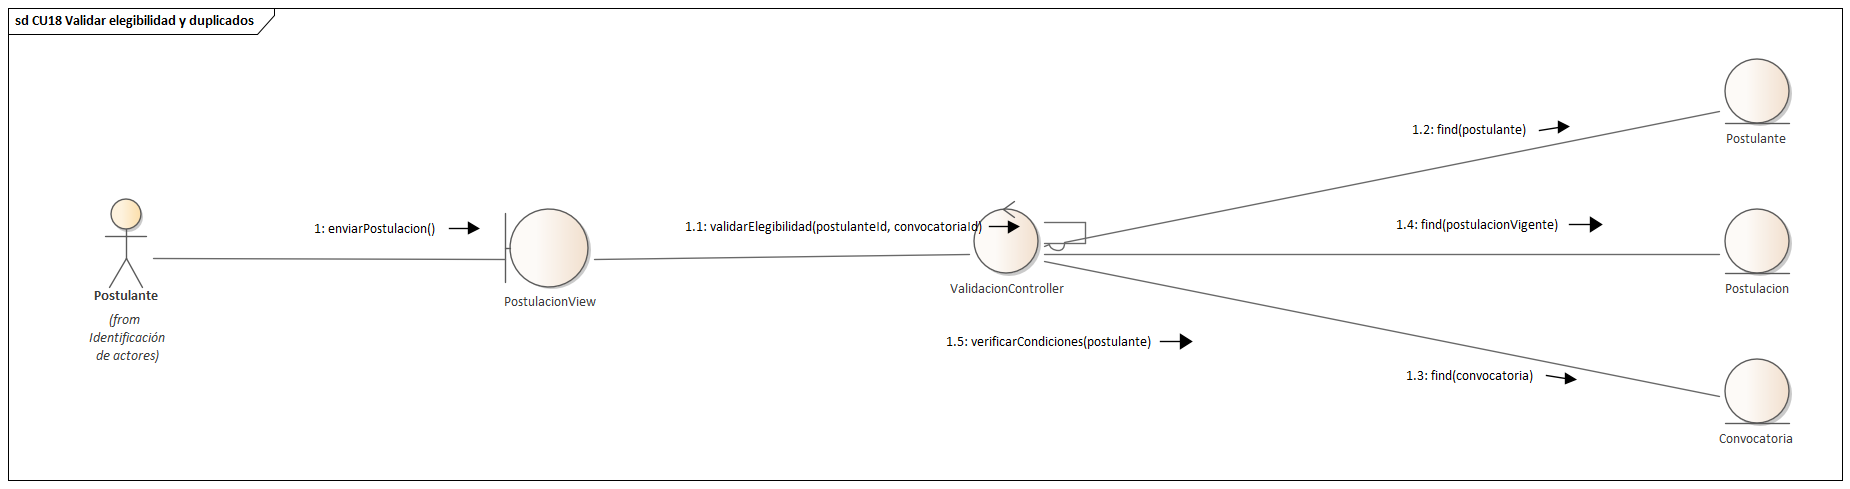
\includegraphics[width=\textwidth,height=0.5\textheight,keepaspectratio]{images/060_Analisis_CU18_Validar_Elegibilidad_Duplicados.png}

\smallskip
\noindent\raggedright\textit{Nota.} Elaboración propia.
\end{figure}

Con la solicitud de validación (mensaje 1.1), el controlador consulta al postulante (1.2), la convocatoria (1.3) y la postulación vigente del postulante en la misma gestión (1.4), y verifica las condiciones de elegibilidad (1.5). El resultado determina si el CU-02 puede registrar la postulación o debe rechazarla indicando el motivo.


\subsubsection{6.2.19. Analizar CU-19 Devolver postulación para corrección}\label{sec:cap6_analisis_cu19}

En el CU-19, el Administrador DUBSS devuelve una postulación mediante \textit{DevolverPostulacionView} y \textit{DevolucionController}, que utiliza las entidades \textit{Postulacion}, \textit{PostulacionHistorial} y \textit{Notificacion}. La Figura~\ref{fig:analisis_cu19} presenta el diagrama de análisis.

\begin{figure}[H]
\caption{Análisis del CU-19 Devolver postulación para corrección}
\label{fig:analisis_cu19}
\centering
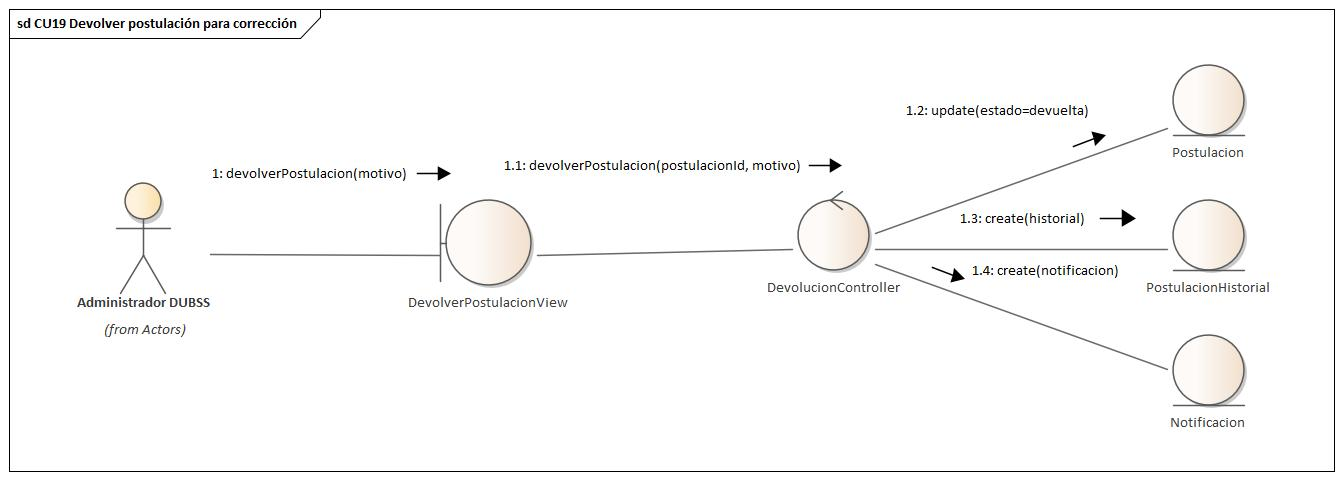
\includegraphics[width=\textwidth,height=0.5\textheight,keepaspectratio]{images/085_Analisis_CU19_Devolver_Postulacion_Correccion.jpg}

\smallskip
\noindent\raggedright\textit{Nota.} Elaboración propia.
\end{figure}

Al devolver la postulación con su motivo (mensaje 1), el controlador actualiza su estado a «devuelta» (1.2), crea el registro del cambio en el historial de la postulación con el motivo (1.3) y crea la notificación dirigida al Postulante (1.4).


\subsubsection{6.2.20. Analizar CU-20 Archivar o rechazar postulación}\label{sec:cap6_analisis_cu20}

En el CU-20, el Administrador DUBSS cierra una postulación mediante \textit{ArchivarPostulacionView} y \textit{ArchivoController}, que trabajan con las entidades \textit{Postulacion} y \textit{PostulacionHistorial}. La Figura~\ref{fig:analisis_cu20} presenta el diagrama de análisis.

\begin{figure}[H]
\caption{Análisis del CU-20 Archivar o rechazar postulación}
\label{fig:analisis_cu20}
\centering
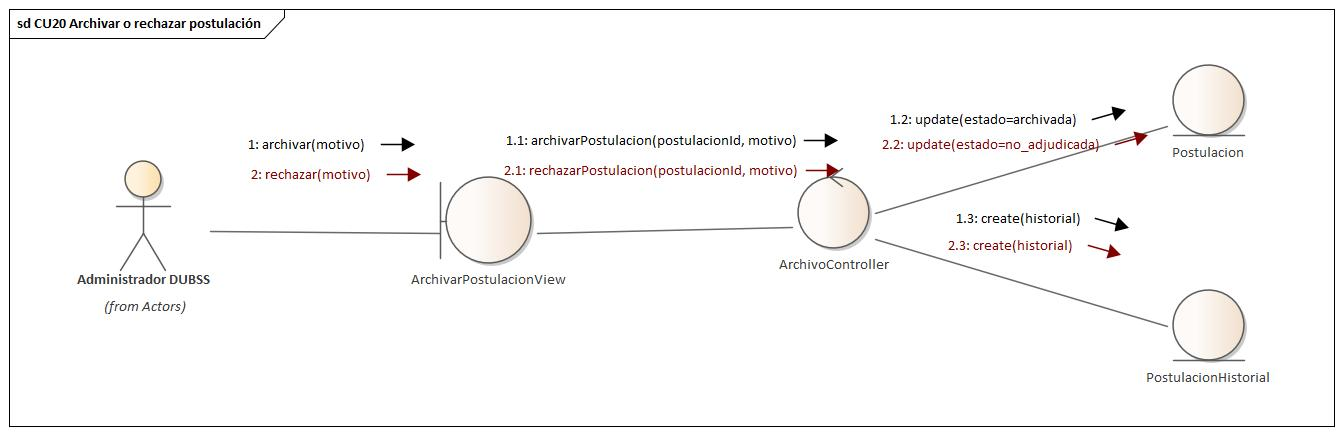
\includegraphics[width=\textwidth,height=0.5\textheight,keepaspectratio]{images/086_Analisis_CU20_Archivar_Rechazar_Postulacion.jpg}

\smallskip
\noindent\raggedright\textit{Nota.} Elaboración propia.
\end{figure}

Al archivar la postulación (mensaje 1), el controlador actualiza su estado a «archivada» (1.2) y registra el cambio con su motivo en el historial (1.3). Al rechazarla (mensaje 2), el controlador actualiza su estado a «no adjudicada» (2.2) y registra igualmente el cambio en el historial (2.3).


\subsubsection{6.2.21. Analizar CU-21 Notificar finalistas, registrar entrega de documentación física y publicar comunicados/avisos}\label{sec:cap6_analisis_cu21}

En el CU-21 participan dos actores: el Administrador DUBSS, que gestiona a los finalistas mediante \textit{FinalistaView}, y el Postulante, que recibe los avisos mediante \textit{AvisoView}. Ambas interfaces se comunican con un único controlador, \textit{NotificacionController}, que utiliza las entidades \textit{Finalista}, \textit{Notificacion} y \textit{Comunicado}. El envío de la notificación push se modela como un mensaje del propio controlador (2.4 y 4.4). La Figura~\ref{fig:analisis_cu21} presenta el diagrama de análisis.

\begin{figure}[H]
\caption{Análisis del CU-21 Notificar finalistas, registrar entrega de documentación física y publicar comunicados/avisos}
\label{fig:analisis_cu21}
\centering
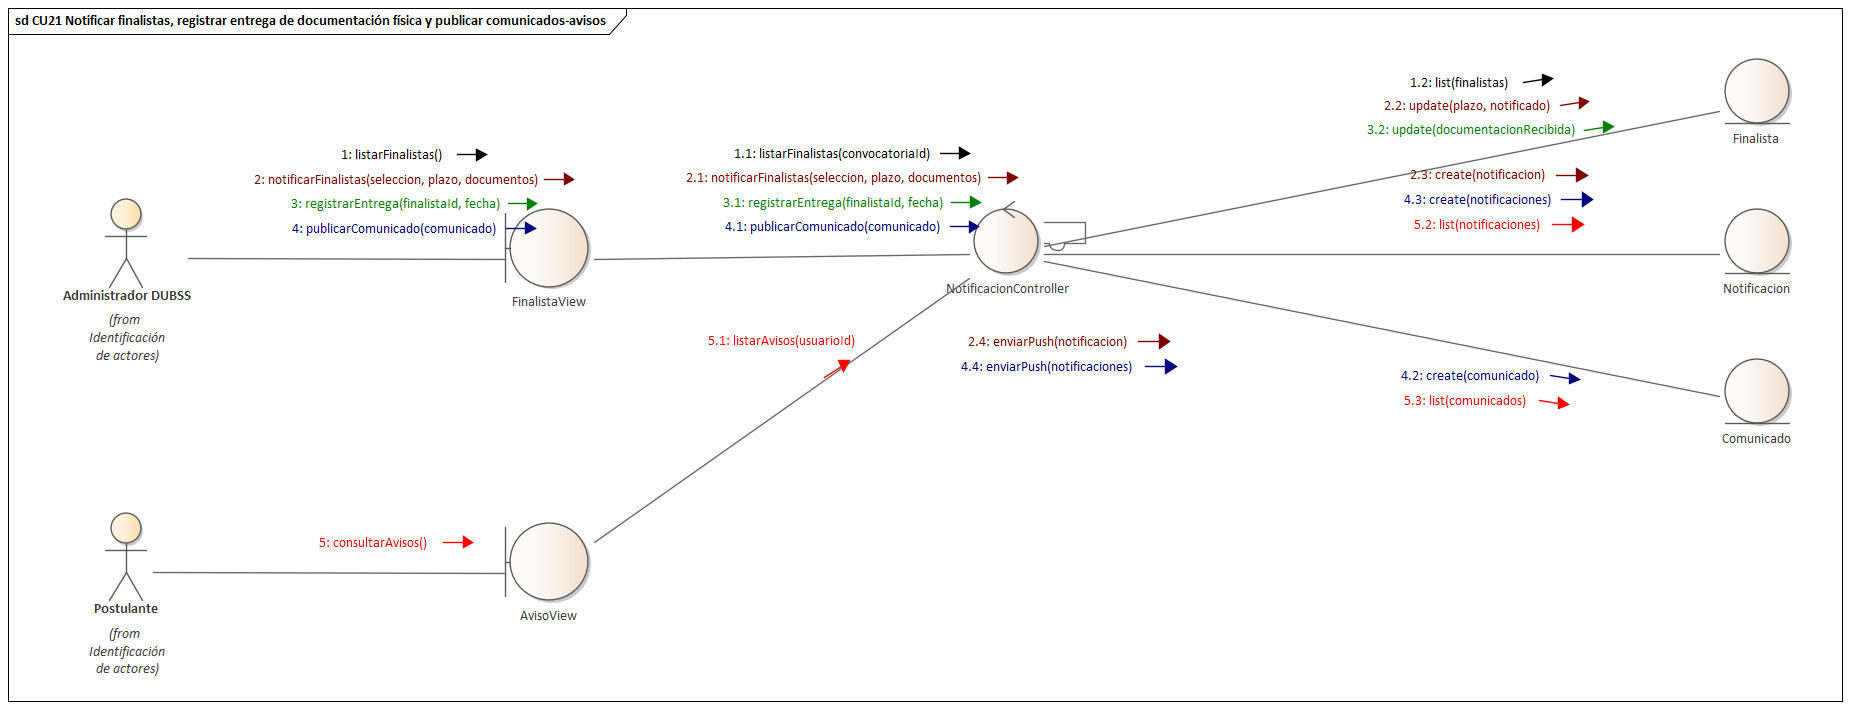
\includegraphics[width=\textwidth,height=0.5\textheight,keepaspectratio]{images/061_Analisis_CU21_Notificar_Finalistas_Publicar_Avisos.png}

\smallskip
\noindent\raggedright\textit{Nota.} Elaboración propia.
\end{figure}

El Administrador puede listar los finalistas (mensaje 1), notificarlos con el plazo y los documentos que deben presentar (mensaje 2), lo que actualiza al finalista (2.2) y crea la notificación (2.3); registrar la entrega de la documentación física (mensaje 3), que actualiza al finalista (3.2); y publicar un comunicado (mensaje 4), que crea el comunicado (4.2) y las notificaciones correspondientes (4.3). El Postulante consulta sus avisos (mensaje 5), con lo que se listan sus notificaciones (5.2) y los comunicados (5.3).


\subsubsection{6.2.22. Analizar CU-22 Publicar resultados de adjudicación}\label{sec:cap6_analisis_cu22}

En el CU-22, el Administrador DUBSS publica los resultados mediante \textit{PublicarResultadosView} y \textit{ResultadosController}, que colaboran con las entidades \textit{Adjudicacion}, \textit{PublicacionResultado} y \textit{Notificacion}. El envío de las notificaciones push se modela como un mensaje del propio controlador (2.4). La Figura~\ref{fig:analisis_cu22} presenta el diagrama de análisis.

\begin{figure}[H]
\caption{Análisis del CU-22 Publicar resultados de adjudicación}
\label{fig:analisis_cu22}
\centering
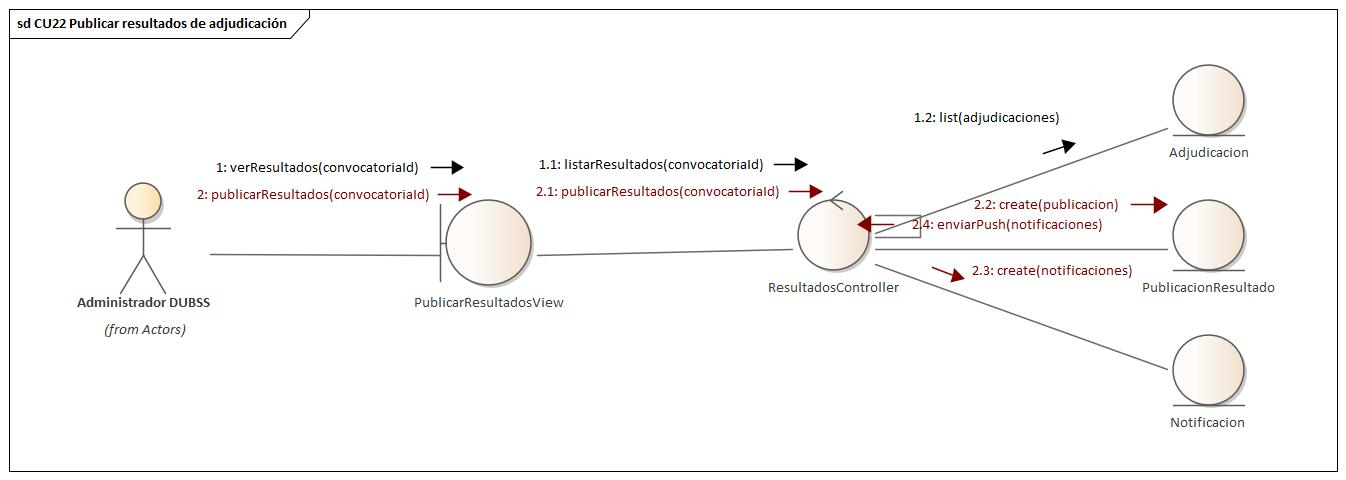
\includegraphics[width=\textwidth,height=0.5\textheight,keepaspectratio]{images/087_Analisis_CU22_Publicar_Resultados_Adjudicacion.jpg}

\smallskip
\noindent\raggedright\textit{Nota.} Elaboración propia.
\end{figure}

Al ver los resultados (mensaje 1), el controlador lista las adjudicaciones de la convocatoria (1.2). Al publicarlos (mensaje 2), el controlador crea el registro de la publicación (2.2), crea las notificaciones dirigidas a los postulantes (2.3) y las envía como notificaciones push (2.4).


\subsubsection{6.2.23. Analizar CU-23 Gestionar padrón de becados (baja, suspensión, reemplazo)}\label{sec:cap6_analisis_cu23}

En el CU-23, el Administrador DUBSS gestiona el padrón mediante \textit{PadronView} y \textit{PadronController}, que utilizan las entidades \textit{Beca} y \textit{MovimientoBeca}. La Figura~\ref{fig:analisis_cu23} presenta el diagrama de análisis.

\begin{figure}[H]
\caption{Análisis del CU-23 Gestionar padrón de becados (baja, suspensión, reemplazo)}
\label{fig:analisis_cu23}
\centering
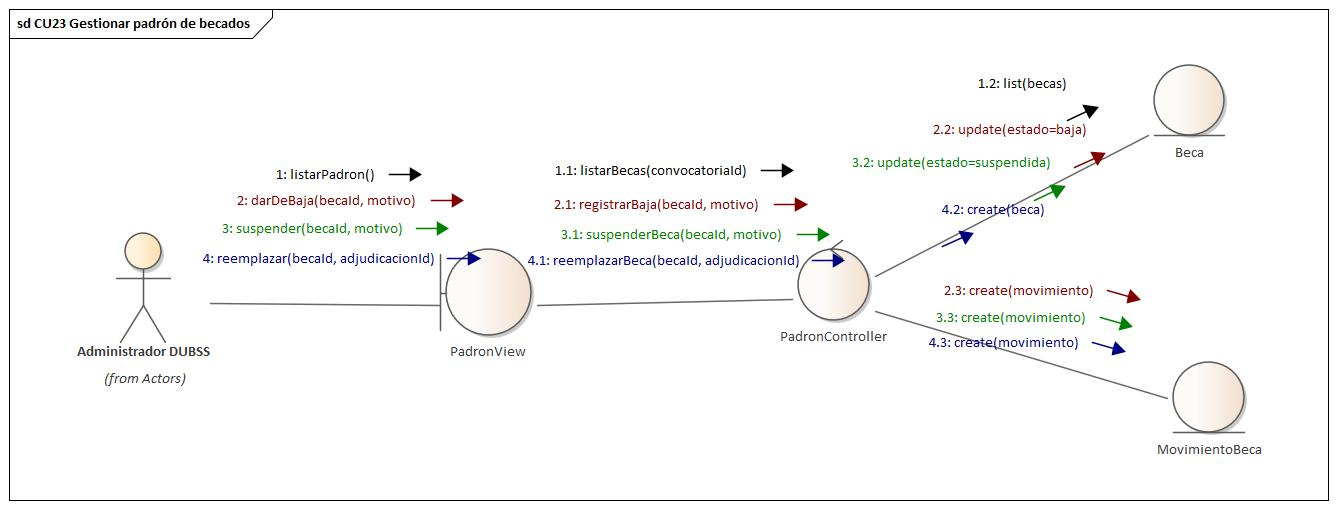
\includegraphics[width=\textwidth,height=0.5\textheight,keepaspectratio]{images/088_Analisis_CU23_Gestionar_Padron_Becados.jpg}

\smallskip
\noindent\raggedright\textit{Nota.} Elaboración propia.
\end{figure}

Al listar el padrón (mensaje 1), el controlador obtiene las becas de la convocatoria (1.2). Al dar de baja una beca (mensaje 2), actualiza su estado a «baja» (2.2) y crea el movimiento correspondiente (2.3). Al suspenderla (mensaje 3), actualiza su estado a «suspendida» (3.2) y crea el movimiento (3.3). Al reemplazar un cupo liberado (mensaje 4), crea una nueva beca para el postulante reemplazante (4.2) y registra el movimiento de reemplazo (4.3).


\subsubsection{6.2.24. Analizar CU-24 Consultar historial de asistencia y estado de beca}\label{sec:cap6_analisis_cu24}

En el CU-24, el Postulante adjudicado (becado) consulta su beca mediante \textit{MiBecaView}, que se apoya en \textit{MiBecaController}. Las entidades involucradas son \textit{Beca}, \textit{MovimientoBeca} y \textit{Asistencia}. La Figura~\ref{fig:analisis_cu24} presenta el diagrama de análisis.

\begin{figure}[H]
\caption{Análisis del CU-24 Consultar historial de asistencia y estado de beca}
\label{fig:analisis_cu24}
\centering
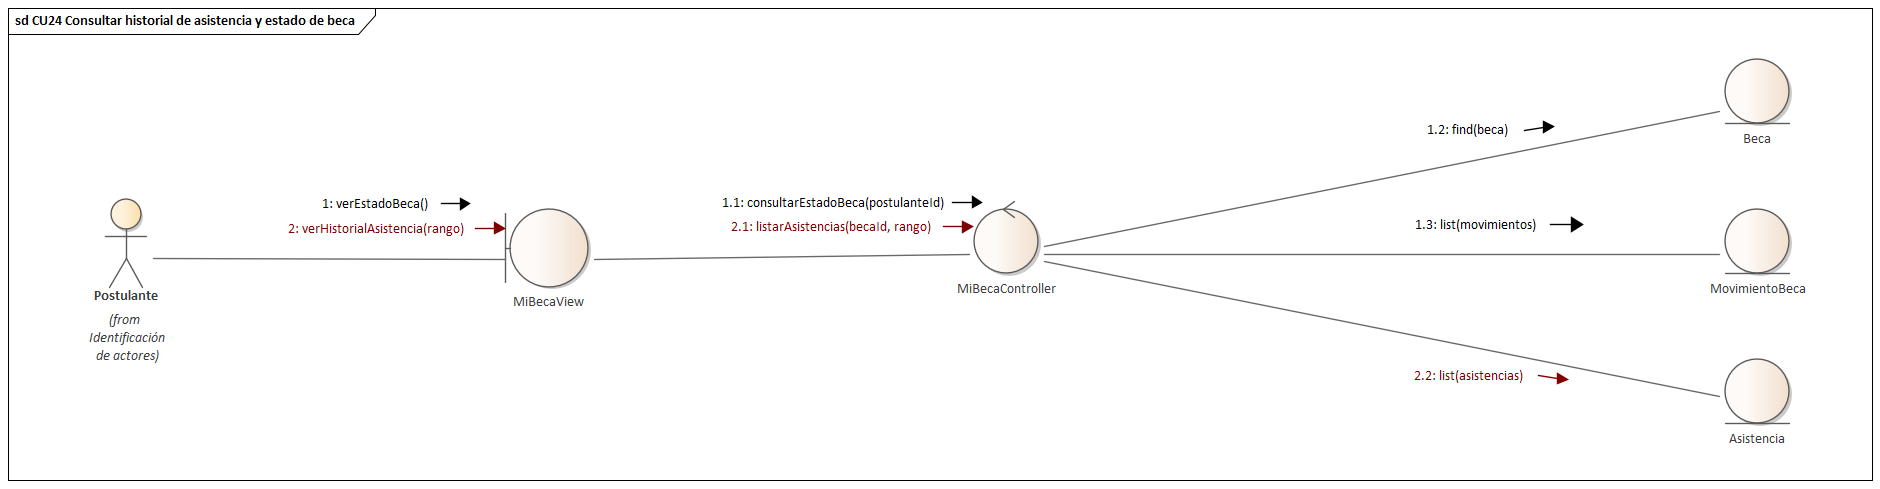
\includegraphics[width=\textwidth,height=0.5\textheight,keepaspectratio]{images/062_Analisis_CU24_Consultar_Historial_Asistencia_Beca.png}

\smallskip
\noindent\raggedright\textit{Nota.} Elaboración propia.
\end{figure}

Para ver el estado de su beca (mensaje 1), el controlador obtiene la beca del postulante (1.2) y sus movimientos de baja, suspensión o reemplazo (1.3). Para ver el historial de asistencia (mensaje 2), lista las asistencias de la beca dentro del rango indicado (2.2). Ambas operaciones son de solo lectura y el becado accede únicamente a su propia información.


\subsubsection{6.2.25. Analizar CU-25 Consultar bitácora de acciones}\label{sec:cap6_analisis_cu25}

En el CU-25, el Administrador DUBSS consulta la bitácora mediante \textit{BitacoraView} y \textit{BitacoraController}. La única entidad involucrada es \textit{Bitacora}, que almacena los registros de las acciones relevantes del sistema. La Figura~\ref{fig:analisis_cu25} presenta el diagrama de análisis.

\begin{figure}[H]
\caption{Análisis del CU-25 Consultar bitácora de acciones}
\label{fig:analisis_cu25}
\centering
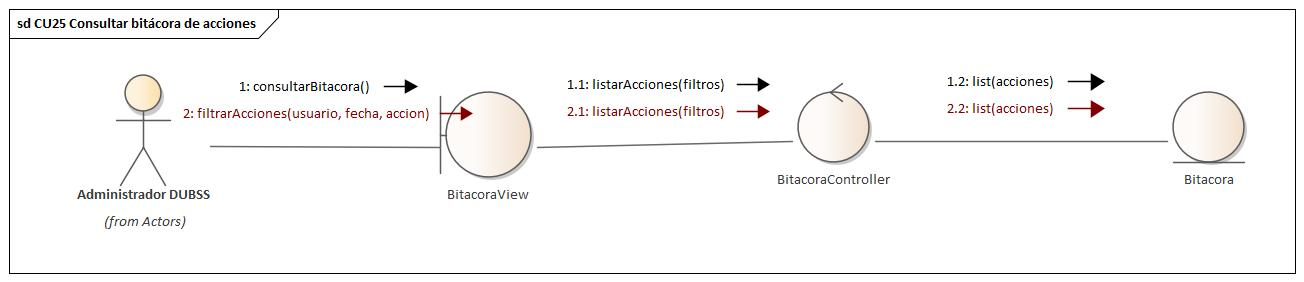
\includegraphics[width=\textwidth,height=0.5\textheight,keepaspectratio]{images/089_Analisis_CU25_Consultar_Bitacora_Acciones.jpg}

\smallskip
\noindent\raggedright\textit{Nota.} Elaboración propia.
\end{figure}

Al consultar la bitácora (mensaje 1), el controlador lista las acciones registradas (1.2). Al filtrar las acciones por usuario, fecha y tipo de acción (mensaje 2), el controlador repite la consulta con los filtros indicados (2.2). Ambas operaciones son de solo lectura y no permiten modificar los registros.


\subsubsection{6.2.26. Analizar CU-26 Parametrizar modelo de preselección y reprocesar puntajes}\label{sec:cap6_analisis_cu26}

En el CU-26, el Administrador DUBSS ajusta el modelo de preselección mediante \textit{ModeloPreseleccionView} y \textit{ModeloPreseleccionController}, que colaboran con las entidades \textit{ModeloPreseleccion}, \textit{ParametroModelo}, \textit{LoteReprocesamiento} y \textit{PuntajePostulacion}. El recálculo de puntajes se modela como el mensaje 3.3 del propio controlador. La Figura~\ref{fig:analisis_cu26} presenta el diagrama de análisis.

\begin{figure}[H]
\caption{Análisis del CU-26 Parametrizar modelo de preselección y reprocesar puntajes}
\label{fig:analisis_cu26}
\centering
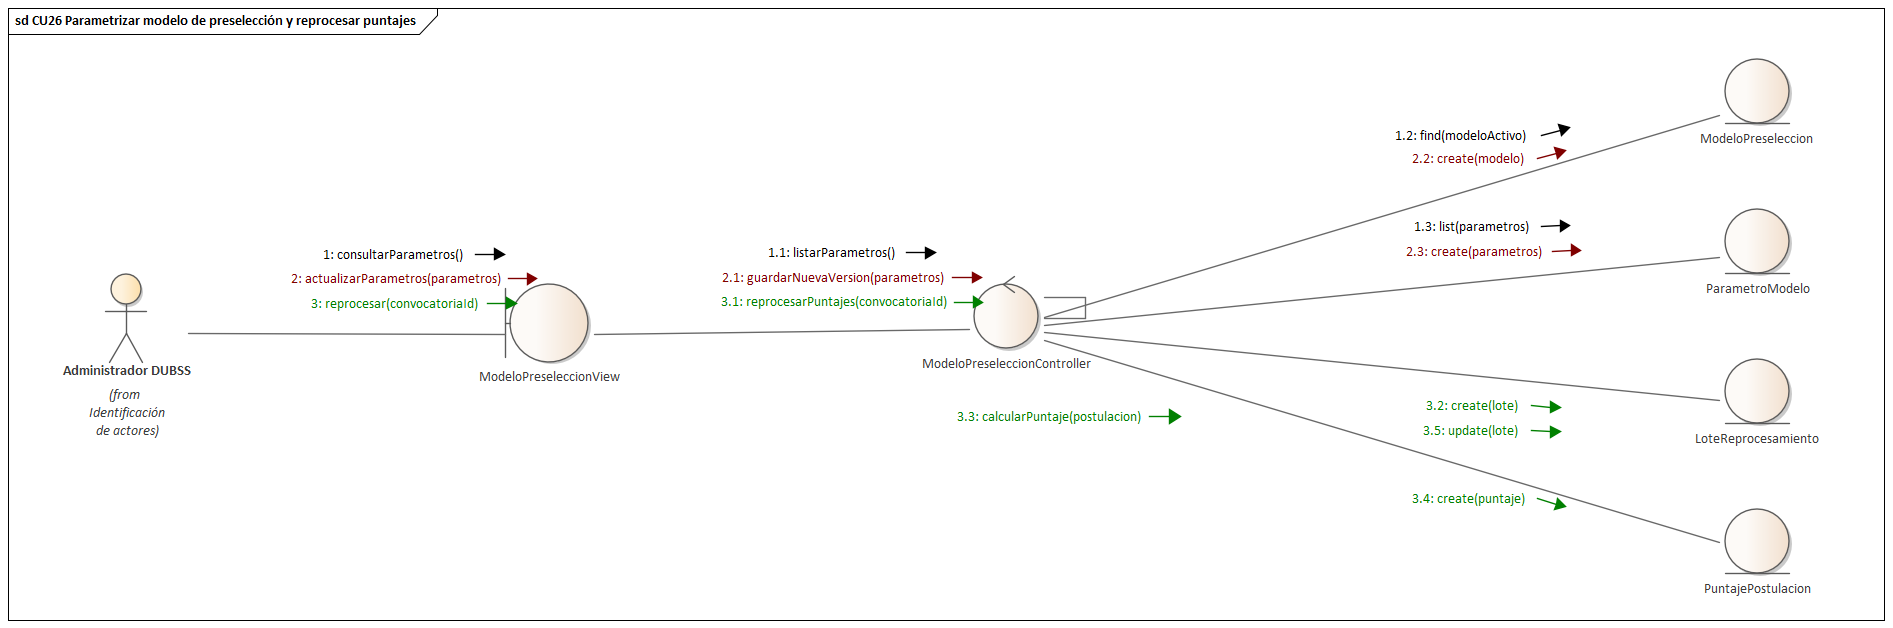
\includegraphics[width=\textwidth,height=0.5\textheight,keepaspectratio]{images/063_Analisis_CU26_Parametrizar_Modelo_Preseleccion.png}

\smallskip
\noindent\raggedright\textit{Nota.} Elaboración propia.
\end{figure}

La consulta de parámetros (mensaje 1) obtiene el modelo activo (1.2) y sus parámetros (1.3). Al actualizarlos (mensaje 2), se crea una nueva versión del modelo (2.2) con sus parámetros (2.3), conservando las versiones anteriores. El reprocesamiento (mensaje 3) crea un lote (3.2), recalcula el puntaje de las postulaciones (3.3), registra los nuevos puntajes (3.4), conservando los anteriores, y actualiza el estado del lote (3.5).

